\documentclass{article}
\usepackage[T1]{fontenc}
\usepackage{lmodern}
\usepackage{graphicx}
\usepackage{amsmath,amssymb}
\usepackage[a4paper,margin=2cm]{geometry}
\usepackage[absolute,overlay]{textpos}
\setlength{\TPHorizModule}{1mm}
\setlength{\TPVertModule}{1mm}
\usepackage[indonesian]{babel}
\usepackage{hyperref}
\setlength{\emergencystretch}{2em}
% unit: Halaman 3

\begin{document}

% === Halaman 3 (llm) ===

\begin{itemize}
  \item Tabel substitusi dapat dibentuk secara acak seperti contoh berikut:
\end{itemize}
\vspace{10mm}
\begin{itemize}
  \item Atau berdasarkan kalimat kunci yang mudah diingat:
\end{itemize}
\textbf{Contoh:} \texttt{di bawah sinar bulan purnama hati resah jadi senang}

\vspace{31.19mm}

\textbf{Buang duplikasi huruf menjadi:} \texttt{dibawhsnrulpmtejg}

\textbf{Sambung dengan huruf lain yang belum ada:}

\texttt{dibawhsnrulpmtejgcfkoqvwxyz}

\textbf{Tabel substitusi yang dihasilkan:}

\begin{tabular}{ll}
Plainteks : & A B C D E F G H I J K L M N O P Q R S T U V W X Y Z \\
Cipherteks : & \textbf{D I B A W H S N R U L P M T E J G C F K O V W X Y Z}
\end{tabular}

% deskripsi: Tabel substitusi huruf acak yang memetakan Plainteks ke Cipherteks
% bbox normalisasi: [0.1900, 0.2050, 0.9050, 0.3100]
\begin{textblock*}{150.15mm}(39.90mm,60.88mm)
\noindent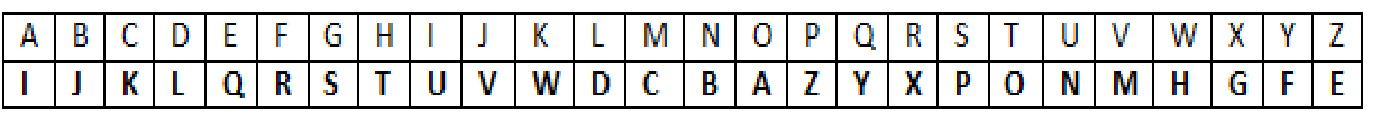
\includegraphics[width=150.15mm,height=31.19mm]{../../images/llm/page_003_img_01.png}%
\end{textblock*}

\end{document}
